\chapter{Kết hợp học sâu với học tăng cường}
\ifpdf
\graphicspath{{Chapter3/Chapter3Figs/PNG/}{Chapter3/Chapter3Figs/PDF/}{Chapter3/Chapter3Figs/}}
\else
\graphicspath{{Chapter3/Chapter3Figs/EPS/}{Chapter3/Chapter3Figs/}}
\fi
\begin{quote}
\textit{Những thành công gần đây của học sâu (Deep learning) trong các bài toán như xử lý ngôn ngữ tự nhiên, nhận diện đối tượng trong ảnh... đặt ra vấn đề: liệu các kỹ thuật trong học sâu có thể áp dụng vào học tăng cường?
Để trả lời câu hỏi đó, chương này trình bày về hướng tiếp cận kết hợp học sâu với học tăng cường để áp dụng vào bài toán ``Tự động chơi game''. 
Hướng tiếp cận mới mẻ này của lĩnh vực học tăng cường này mang tên ``Học tăng cường sâu'' (Deep reinforcement learning)\\
Chương này trình bày hai phần:
\begin{itemize}
	\item Nguyên nhân cần sử dụng học sâu và kiến thức cơ bản về học sâu
	\item Áp dụng học tăng cường sâu vào bài toán ``Tự động chơi game''
\end{itemize}}
\end{quote}

\section{Học sâu}
\subsection{Khó khăn của bài toán tự động chơi game}
	Những thuật toán học tăng cường được trình bày trong chương trước đều tìm chính sách tối ưu dựa vào hàm giá trị. 
	Việc tính \textbf{đúng} và \textbf{nhanh} hàm giá trị ảnh hưởng rất nhiều đến kết quả của bài toán. 
	Các thuật toán học tăng cường cổ điển như ``Monte Carlo'' (MC) hay ``Temporal-Difference'' (TD) đều đã được chính minh là luôn hội tụ trong những điều kiện nhất định \cite{sutton1998introduction}. 
	Ngoài ra, khi áp dụng vào các bài toán kinh điển của học tăng cường thì các thuật toán này đều hội tụ khá nhanh.
	
	Tuy nhiên, với những bài toán thực tế với số trạng thái rất lớn thì việc lưu véc-tơ hàm giá trị trạng thái $v_{\pi}$ (hoặc ma trận hàm giá trị hành động $q_{\pi}$) là việc không thể. 
	Ví dụ như ``frame hình'' của bài toán tự động chơi game có kích thước $210\times160\times3=100800$ điểm ảnh; mỗi điểm ảnh có giá trị trong khoảng $[0, 127]$ nên số trạng thái có thể có lên đến $128^{100800}$.
	Vì vậy, việc lưu trữ hàm giá trị dưới dạng bảng là không khả thi về mặt bộ nhớ.
	Còn về mặt tốc độ tính toán thì các thuật toán học tăng cường trên đều tính hàm giá trị \textit{rời rạc} cho từng trạng thái.
	Với số trạng thái quá lớn như trên thì ta không thể duyệt lần lượt từng trạng thái để tính được.
	
	Những lý do trên dẫn đến việc sử dụng một phương pháp xấp xỉ hàm là bắt buộc cho các bài toán học tăng cường với số trạng thái lớn.
	Một trong những tiếp cận rất tự nhiên đó là sử dụng các mô hình học có giám sát như là một phương pháp xấp xỉ hàm giá trị.
	Đặc biệt, với những đột phá gần đây của học sâu trong lĩnh vực xử lý ảnh, video... thì việc áp dụng các mô hình phổ biến của học sâu vào bài toán tự động chơi game là đầy hứa hẹn.
	
\subsection{Giới thiệu học sâu}
	Các mô hình truyền thống trong lĩnh vực máy học như ``Linear regression'', ``Bayesian learning''... thông thường đều hoạt động trên các đặc trưng được \textit{rút trích một cách thủ công} (hand-designed features).
	Với dữ liệu thô thu thập được từ thực tế, các nhà khoa học xây dựng các phương pháp rút trích ra những ``thông tin hữu ích'' (thường được gọi là đặc trưng) để cung cấp cho các mô hình máy học.
	Kết quả nhận được từ các mô hình này phụ thuộc rất lớn vào cách biểu diễn dữ liệu.
	Ví dụ như trong bài toán nhận diện người nói từ một đoạn âm thanh, các đặc trưng có thể bao gồm: độ lớn âm thanh, tần số trung bình của đoạn âm,...
	Nếu các đặc trưng này không đủ ``mạnh'' (như có hai người nói đoạn âm thanh nhưng lại có chung độ lớn, tần số...) thì các mô hình học sẽ không thể phân biệt.
		
	Để giải quyết vấn đề thiết kế đặc trưng, các mô hình máy học thuộc loại ``Học biểu diễn'' \textit{(Representation learning)} ra đời.
	Các mô hình này có khả năng tự động học luôn các đặc trưng cần thiết cho quá trình phân tích dữ liệu.
	Nhờ vậy, các mô hình này có thể áp dụng được dễ dàng hơn vào các bài toán thực tế mà không cần con người phải can thiệp.
	Tuy nhiên, các đặc trưng cần thiết lại có thể rất phức tạp.
	Việc học ra các đặc trưng này có thể khó ngang với việc giải bài toán gốc.
	Ví dụ như trong bài toán nhận diện người nói trên, ta có thể sử dụng thông tin về giọng địa phương của người nói (accent).
	Đặc trưng này rất trừu tượng, không dễ phân tích bằng máy tính mặc dù con người có thể nhận biết một cách khá dễ dàng.
	Vì vậy, nếu các đặc trưng cần thiết quá khó để học thì các mô hình máy học thuộc loại ``Học biểu diễn'' cũng không thể cho kết quả tốt.

	Học sâu (Deep learning) được ra đời nhằm giải quyết các vấn đề trên.
	Học sâu là một nhánh của ``Học biểu diễn'' nên vẫn có thể tự động học ra các đặc trưng hữu ích.
	Học sâu được thiết kế để học ra các đặc trưng có quan hệ với nhau theo nhiều tầng (layer).
	Các đặc trưng ở tầng phía sau được xây dựng dựa vào các đặc trưng ở tầng phía trước.
	Các tầng đầu tiên bao gồm những đặc trưng đơn giản và các tầng tiếp theo ngày càng trừu tượng, ngày càng phức tạp hơn.
	Mỗi tầng chỉ cần học cách xây dựng đặc trưng từ những đặc trưng ở tầng phía trước (đã có sẵn độ trừu tượng nhất định) thay vì học từ dữ liệu thô ban đầu; điều này giúp cho học sâu có khả năng học được những đặc trưng rất phức tạp.
	
	\begin{figure}
		\centering
		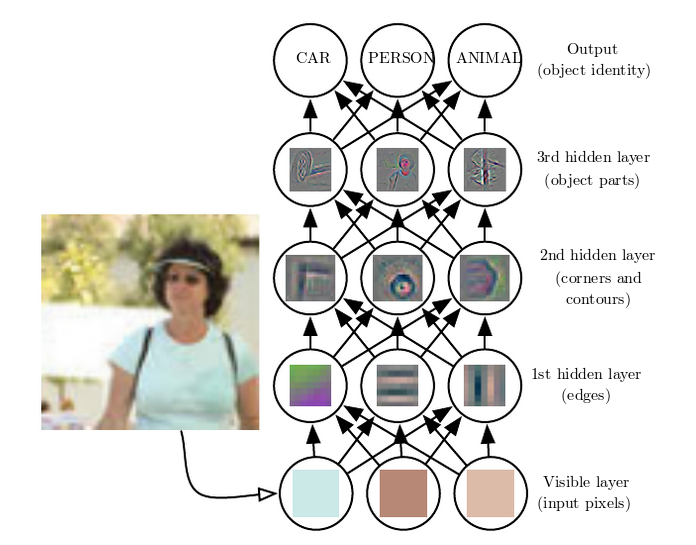
\includegraphics[width=\textwidth]{deep_learning_example}
		\caption{Hình mô phỏng cách hoạt động của mô hình học sâu cho bài toán nhận diện đối tượng trong ảnh.
		Dữ liệu đầu vào là hình ảnh RGB chứa đối tượng cần xác định. Tầng đầu tiên của mô hình là tầng ``input'' tiếp nhận thông tin này dưới dạng ma trấn số. 
		Các tầng tiếp theo ngoại trừ tầng cuối cùng được gọi là tầng ẩn ``hidden layer'' vì đặc trưng học được tại đây con người không quan sát được. 
		Các tầng ẩn học các đặc trưng ngày càng trừu tượng dựa vào đặc trưng ở tầng phía trước. 
		Tầng ẩn đầu tiên học được các đặc trưng về cạnh bằng cách so sánh độ sáng giữa các điểm ảnh gần nhau. 
		Tầng ẩn thứ hai học được các đặc trưng về đường cong bằng cách tổng hợp đặc trưng về cạnh ở tầng trước đó. 
		Tầng ẩn thứ ba học được các đặc trưng về bộ phận của đồ vật như khuôn mặt, bánh xe... dựa vào các đặc trưng về đường cong ở tầng trước. 
		Tầng cuối cùng được gọi là tầng ``output'' có nhiệm vụ tìm kiếm các bộ phận và trả về lớp đối tượng tương ứng. 
		Bằng cách học đặc trưng ngày càng trừu tượng hơn, các mô hình học sâu có khả năng tự động học được các đặc trưng từ đơn giản đến phức tạp; tất cả đều nhằm hỗ trợ cho quá trình phân lớp dữ liệu (hình được chỉnh sửa từ \cite{Goodfellow-et-al-2016-Book})}
		\label{dlex}
	\end{figure}
	
\subsection{Áp dụng học sâu để xấp xỉ hàm giá trị}
	Sức mạnh của các mô hình học sâu hoàn toàn có thể tận dụng vào bài toán học tăng cường.
	Cụ thể với những thuật toán học tăng cường được đề cập ở chương 2, việc xấp xỉ hàm giá trị là rất quan trọng.
	Chính vì vậy, một cách đơn giản nhất, ta có thể sử dụng các mô hình học sâu để xấp xỉ hàm giá trị.
	Một trong những mô hình tiêu biểu của học sâu đó là mạng nơ-ron (Neural networks).
	Việc sử dụng mạng nơ-ron để xấp xỉ hàm giá trị mang lại ba lợi ích quan trọng:
	\begin{itemize}
		\item Mạng nơ-ron có khả năng học được những đặc trưng phức tạp từ dữ liệu thô.
		\item Mạng nơ-ron có thể xấp xỉ hàm giá trị phức tạp.
		\item Mạng nơ-ron có tính tổng quát hoá.
	\end{itemize}
	
	Mạng nơ-ron là một mô hình học sâu nên có thể học được những đặc trưng phức tạp từ dữ liệu thô như đã nói ở phần trên.
	Cụ thể hơn trong bài toán tự động chơi game, ta có thể đưa dữ liệu đầu vào là các ``frame hình'' RGB thẳng vào ``input'' của mạng nơ-ron để tính ra giá trị tương ứng.
	Nhờ vậy, ta không cần phải thiết kế các đặc trưng bằng tay để biễu diễn cho từng trạng thái của game.
	Ngoài ra, do qua trình học đặc trưng là hoàn toàn tự động, thuật toán học tăng cường lúc này có thể áp dụng cho bất kỳ game nào mà không cần phải thay đổi cách rút trích đặc trưng.
	Với một mô hình cố định lúc này, ta có thể học chơi được nhiều game.
	Đây cũng chính là mục đích của bài toán tự động chơi game: xây dựng mô hình có khả năng tự động học chơi \textit{tốt} nhiều game chứ không chỉ chơi \textit{``hoàn hảo''} một game.
	
	Với bài toán tự động chơi game, giá trị của một trạng thái bất kỳ rất khó xác định do một màn game thường rất dài.
	Vì thế, hàm giá trị của bài toán này là một hàm phi tuyến phức tạp và không liên tục.
	Công cụ xấp xỉ hàm giá trị phải có khả năng xấp xỉ những hàm phức tạp như vậy thì thuật toán học tăng cường mới đạt được hiệu quả.
	Với cách nhìn nhận mạng nơ-ron như là một công cụ xấp xỉ hàm, ta có thể thấy mạng nơ-ron rất linh hoạt với khả năng xấp xỉ hàm đích bất kỳ.
	
	Một tính chất quan trọng khác của mạng nơ-ron chính là \textbf{khả năng tổng quát hoá} (Generalization).
	Nhờ đặc điểm này mà quá trình học tăng cường được tăng tốc đáng kể.
	Thay vì phải duyệt qua từng trạng thái (thậm chí phải duyệt nhiều lần) để tính hàm giá trị tại đó, mạng nơ-ron có khả năng ``dự đoán'' giá trị của một trạng thái chưa từng thấy dựa vào những trạng thái đã thấy.
	Như trong bài toán tự động chơi game thì các ``frame hình'' liên tiếp thường rất giống nhau và các trạng thái này thường cũng có giá trị tương đương nhau.
	Vì vậy, khi học xong cách chơi một game nào đó, thuật toán học tăng cường vẫn hoạt động tốt trong quá trình kiểm thử khi gặp những tình huống game chưa từng thấy trong lúc huấn luyện.
	
	Các thuật toán học tăng cường ở chương 2 đều lưu hàm giá trị dưới dạng bảng (lookup table).
	Để sử dụng mạng nơ-ron như một công cụ xấp xỉ hàm, lúc này ta coi hàm giá trị là một hàm có tham số (parameterized function) và đi tìm các tham số này:
	\begin{align}
		\hat{v}(s;\theta) &\approx v_{\pi}(s)\\
		\hat{q}(s,a;\theta) &\approx q_{\pi}(s,a)
		\label{eq_DefVhatQhat}
	\end{align}
	$\theta$ là bộ trọng số của mạng nơ-ron mà ta cần học.
	Để học được bộ trọng số xấp xỉ tốt hàm đích ($v_{\pi}(s)$ hoặc $q_{\pi}(s,a)$), ta cung cấp các mẫu dữ liệu (data sample).
	Mỗi mẫu bao gồm dữ liệu đầu vào của mạng nơ-ron (tức trạng thái $s$ hoặc bộ trạng thái, hành động $s, a$) cùng với giá trị đích mong muốn (tức $v_{\pi}(s)$ hoặc $q_{\pi}(s,a)$).
	Khi ta cung cấp đủ nhiều mẫu dữ liệu cho mạng nơ-ron, các bộ tham số sẽ được thay đổi để mạng xấp xỉ được hàm đích mong muốn.
	Số lượng mẫu dữ liệu càng lớn thì mạng nơ-ron càng ``thấy'' được nhiều giá trị tại nhiều vị trí khác nhau của hàm đích hơn, khi đó mạng nơ-ron càng có khả năng xấp xỉ hàm đích tốt hơn.	
	Để xét xem mạng nơ-ron có xấp xỉ tốt hàm đích hay chưa, ta có thể tính độ ``khác biệt'' của giá trị đích với giá trị xấp xỉ trên cả không gian đầu vào:
	\begin{align}
		J(\theta) &= \mathbb{E}_{s \sim \pi}[(v_{\pi}(s) - \hat{v}(s;\theta))^2]\\
		J(\theta) &= \mathbb{E}_{s,a \sim \pi}[(q_{\pi}(s,a) - \hat{q}(s,a;\theta))^2]
		\label{eq_ExpectedError}
	\end{align}
	Kỳ vọng $\mathbb{E}_{s \sim \pi}$ ý chỉ kỳ vọng với biến ngẫu nhiên là trạng thái $s$ được lấy từ phân bố do chính sách $\pi$ tạo nên.
	Ví dụ như ta cần xấp xỉ hàm giá trị của một chính sách chỉ luôn ``đi qua trái'' thì $s$ sẽ là những trạng thái mà khi đi theo chính sách này, ta có thể gặp được $s$.
	Trong khi đó nếu chính sách đang xét là ``đứng yên'' (không thay đổi trạng thái) thì $s$ chỉ có thể có một trạng thái duy nhất đó là trạng thái bắt đầu.
	Giá trị nằm trong kỳ vọng là độ lỗi bình phương giữa giá trị xấp xỉ và giá trị đích.
	Với hàm lỗi bình phương, có thể thấy khi $J(\theta)$ càng nhỏ thì bộ trọng số $\theta$ giúp cho mạng nơ-ron xấp xỉ hàm đích càng tốt.
	Lý do chính ta chọn độ lỗi bình phương (ví dụ thay vì độ lỗi theo trị tuyệt đối) là vì việc tính toán (như đạo hàm) trên hàm bình phương khá dễ dàng.
	
	Lưu ý là ở đây, hàm lỗi $J(\theta)$ là hàm theo $\theta$; tức là lúc này, ta cố định bộ trọng số $\theta$ để tìm ra ``sai số'' mà bộ trọng số này gây ra.
	Nếu ta có hai bộ trọng số $\theta_1$ và $\theta_2$, ta có thể so sánh khả năng xấp xỉ hàm đích của chúng bằng cách so sánh giá trị $J(\theta_1)$ và $J(\theta)_2$ tương ứng.
	
	Tuy nhiên ta không thể tính độ lỗi trên mọi điểm dữ liệu đầu vào theo công thức (\ref{eq_ExpectedError}) được vì số lượng trạng thái là rất lớn.
	Vậy ta có thể xấp xỉ giá trị $J(\theta)$ bằng cách chỉ xét độ lỗi trên một ``tập huấn luyện'' (hay còn gọi là ``Batch'') các trạng thái mà ta biết được giá trị đích.
	Khi đó, kỳ vọng $\mathbb{E}_{s \sim \pi}$ được thay thế bằng giá trị trung bình độ lỗi trên từng mẫu dữ liệu của ``batch'':
	\begin{align}
		J(\theta) &= \frac{1}{N} \sum_{i = 1}^{N}[(v_{\pi}(s_{i}) - \hat{v}(s_{i};\theta))^2]\\
		J(\theta) &= \frac{1}{N} \sum_{i = 1}^{N}[(q_{\pi}(s_i,a_i) - \hat{q}(s_i,a_i;\theta))^2]
		\label{eq_BatchError}
	\end{align}
	Trong đó:
	\begin{itemize}
		\item N là số mẫu dữ liệu trong ``batch''.
		\item $s_i$, $a_i$ tương ứng là trạng thái và hành động của mẫu dữ liệu thứ $i$ của ``batch''.
	\end{itemize}
	Với một tập huấn luyện bất kỳ (tức một ``batch''), ta mong muốn tìm được bộ trọng số giúp cho mạng nơ-ron xấp xỉ tốt hàm đích trên các mẫu dữ liệu thuộc tập huấn luyện này.
	Một thuật toán đơn giản và hay được sử dụng để tìm bộ trọng số này đó là ``Batch Gradient Descent'' (BGD).
	Để cực tiểu hoá hàm $J(\theta)$, thuật toán BGD thực hiện lặp lại nhiều ``bước đi'' nhỏ để thay đổi bộ trọng số $\theta$ dần dần; mỗi bước đi sẽ giúp cho hàm $J(\theta)$ giảm đi một ít.
	Để chọn ``hướng đi'' (tức cách cập nhật $\theta$) thì BGD sẽ ``nhìn'' xung quanh vị trí hiện tại và đi theo hướng nào giúp giảm $J(\theta)$ nhiều nhất có thể.
	
	
	Tuy nhiên, giá trị đích thực sự mà ta mong muốn là $v_{\pi}(s)$ (hoặc $q_{\pi}(s,a)$) ta không hề biết.
	Các thuật toán học tăng cường chính là kỹ thuật giúp ta có được một ước lượng đơn giản của giá trị đích này.
	

%\begin{itemize}
%	\item Lý do kết hợp học sâu với học tăng cường
%	\item Giới thiệu học sâu
%	\item Áp dụng học sâu để xấp xỉ hàm giá trị
%	\item Giới thiệu mạng ``Convolutional Neural Network''
%\end{itemize}
	
\section{Học tăng cường sâu}
%\begin{itemize}
%	\item Cấu trúc mạng ``Deep Q-Networks'' cho bài toán tự động chơi game
%	\item Kỹ thuật làm tăng tính ổn định cho quá trình học
%	\begin{itemize}
%		\item Học từ dữ liệu trong quá khứ ``Experience replay''
%		\item Cố định hàm giá trị đích ``Fixed Q-targets''
%	\end{itemize}
%\end{itemize}
%	
%\section{Đề xuất phương pháp cải tiến (Nếu có)}
	